\chapter{Model development}
\label{chap:ModelDevelopment}
This chapter will discuss the simulation model used for the evaluation of the option pricing techniques. \todo{descr} 

\section{Simulation model}
In this paper a series of simulations will be run to determine the performance of the proposed option valuation models. The simulation model will calculate the expected profits or losses of each of these models. To do so, it will run through a number of steps, namely:

\begin{description}
\item[Generate passengers] the simulation model will generate a single passenger for each day prior to departure of a specific flight. Because data have been collected on flights up till 42~days before departure, each ticket will receive this same number of passengers with option requests. However, because when selling options with a specific number of days to maturity $m$ it is not possible to buy options fewer that $m$ days to departure, these customers get excluded from the model. As an example, the test dataset containing airfares of tickets from LHR to JFK includes 7,690 unique flights after cleansing. When simulating this model for options with a maturity of 3 days a total of $(42 - 3) \times 7,690 = 299,910$ passengers will be generated.
\item[Calculate the passenger's WTP] the passenger's \emph{Willingness To Pay} is determined by calculating the minimum costs incurred when buying the flight immediately or waiting to buy the ticket at maturity. A more complete explanation of this concept can be found in \typenameref{subsec:PassengersWTP}. For the simulation the equation takes into account several properties of a passenger. These parameters are \begin{inparaenum}[\itshape (i)\upshape]
    \item risk-utility,
    \item forecasting technique, and
    \item likelihood of travelling.
\end{inparaenum} The implementation of these concepts is explained in detail in \todo{ref}.
\item[Calculate the option seller's WTA] the \emph{Willingness To Accept} of an option according to the external party is calculated using its predictions of how the airfare is expected to change. This variable is dependant upon two parameters, namely: \begin{inparaenum}[\itshape (i)\upshape]
    \item Forecasting technique, and
    \item information transparency.
    \end{inparaenum} These parameters will be described in detail in \todo{ref}.
\item[Compare the WTP with the WTA] by comparing the customer's WTP and the seller's WTA, the model can determine whether the customer will buy the offered option. This is the case when the Willingness To Pay of the customer for a certain flight is higher than the Willingness To Accept of the seller (i.e., $\text{WTP} \ge \text{WTA}$).
\item[Sell the option] when the customer will buy the option, the simulation will ``sell'' the option at the specified price.
\item[Calculate generated profits] when an option is sold to a passenger, the model first checks whether the customer actually wants to exercise its right on the day of maturity. A customer will only exercise its right when he is actually flying, and the airfare on the date of maturity is higher than the strike price $p_s$. When this is the case, the simulation will compare the airfare at maturity with the strike price, and calculate the profits or losses resulted from the sale of the product. In this paper the strike price of the option is equal to the airfare at the moment of offering the airfare~lock-in product.
\end{description}

\noindent
This whole process of the simulation model is summarized in \todo{ref}.

\todo[illustration]{Illustration of process}

Using the method described above, the simulation will be used to compare the performance of the proposed option valuation models amongst each other. The same procedure will also be used to test the influence of a particular configuration of parameters within a single option valuation model.


\todo{descr the first case in words: allknowing foreknowledge..}

\subsection{Parameters and assumptions of the simulation model}
For this simulation, a number of parameters have been defined and some assumptions have been made. The next section will describe the base case which is being used for the initial simulation. In this portion, the exact configurations of the parameters and assumptions will be described. Later sections (e.g., \todo{ref}) will loosen the specified parameters to see its effects on the performance of the parameters itself.

Like in \typenameref{sec:Entities}, this model will categorize the parameters and assumptions according to their underlying entities. These four sections are \begin{inparaenum}[\itshape (i)\upshape]
\item the flight~ticket,
\item the airfare~lock-in product,
\item the option seller, and
\item the passenger.
\end{inparaenum} Each of these entities has its own set of characteristics, which will be defined below.

\subsubsection{Characteristics of the flight ticket}
\label{sub:CharacteristicsOfTheFlightTicket}
The first entity represents the flight~ticket. A ticket gives its holder the right to take a seat on a particular underlying flight. In this thesis, a specific set of flights is being used:

\begin{itemize}
\item each flight is for a specific route between outbound and inbound airport;
\item only single-legged (direct) flights are being considered;
\item only round trip flights are being considered;
\item each flight has a specific departure date;
\item the return date of the flight is always 1~week after the departure date.
\end{itemize}

Each ticket also has a certain price. This price can differ depending on the lookup~time of the ticket. In this research, airfare changes have been monitored up to six~weeks prior to departure. A certain price of a ticket can thus be defined in the number of \emph{days before departure}, or \emph{dbb}.

This thesis has collected airfares on flight tickets for 22~different routes during a period of 12~weeks. The empirical data acquired in this stage are being used in the simulation model. The complete analysis on these airfares is given in \autoref{chap:DataAnalysis}.

\subsubsection{Characteristics of the airfare~lock-in product}
The next entity which is being considered in this simulation model is the airfare~lock-in product. This product gives its holder the right --- but not the obligation --- to buy the underlying flight. There are two parameters associated with the entity.

\parameter{the option's number of days till maturity \hfill ($m = 3$)}
The first parameter of the airfare~lock-in products is its number of days till maturity. This value denotes the number of days of extra \emph{decision time} a customer gains when he buys the option. At the date of maturity, the customer has to make the decision to actually buy the ticket, or to not exercise the option at all. A passenger will choose for the first alternative when he has decided to actually fly, and the current airfare is higher than the agreed upon \emph{strike price}. During this number of days $m$, the customer is thus \emph{insured} against price fluctuations and will therefore not risk high fare increases.

In the base case for the simulation, a maturity of 3~days is being considered. When a passenger thus purchases the option, he will decide whether to exercise the option 3~days after the acquisition of the lock-in product.

\parameter{the option's strike price \hfill ($p_S = p_I$)}
The second parameter is the strike price of the airfare~lock-in product. This price, denoted by $p_S$, is the cost at which the passenger is able to buy the underlying flight ticket when he exercises the option.

This research will consider a strike price of the airfare~lock-in product that is equal to the initial airfare of the underlying flight at purchase of the option.

$$p_S = p_I$$

For example, when the current ticket price $p_I$ is equal to \$\,100 and the customer decides to buy the option, he has the opportunity to buy the ticket for \$\,100 at the date of maturity.  

Next to these configurable parameters, an airfare~lock-in product also has a certain price at which the option is offered to the customer. The theoretical level of this option price is described in \typenameref{subsec:PassengersWTP}. In this research, however, three different option valuation techniques are being considered. These pricing models are characterized by different configurations of the parameters of this simulation model, and will be described in \typenameref{chap:DataAnalysis}.

\assumption{the option's maximum price \hfill ($p_O \le 0.15 \times p_I$)}
An assumption made about the simulation model in this thesis, is that option prices will not exceed 15~percent of the initial airfare:

$$p_O \le 0.15 \times p_I$$

This assumption is made to exclude the possibility of exceptionally high option prices due to inaccurate forecasts of the passenger. During test~runs of the simulation model, option prices sometimes appeared to be as high as 50~percent of the current ticket price. This seems to be a to high estimation, and these outliers have to be re-evaluated. The 15~percent level as a maximum seems like a realistic maximum for option prices in a real setting.


\subsubsection{Characteristics of the options seller}
Another entity considered in the simulation model of this research is the seller of the airfare~lock-in products. This is the object that offers the options to the customer. The simulation model described also has associated some parameters and assumptions to this entity.

\parameter{the seller's forecasting technique \hfill (foreknowledge)}
In accordance with the theoretical minimum option price as described in \typenameref{subsec:PassengersWTP}, the option seller has to make predictions on the fluctuation of the airfare. The seller will only sell an option to the passenger, when he expects that the losses of exercising the option are lower than the gains from selling the airfare~lock-in product. The seller will therefore gain from having more accurate forecasting models that predict future airfares closer to the actual observed value.

The base model of simulation will consider an option seller with foreknowledge. This theoretical forecasting method assumes that when the seller offers an option to the passenger, the writer already knows what the airfare will be at the date of maturity. The seller thus is able to forecast prices with 100~percent accuracy. While this is a theoretical case, it will offer insights in the maximum profits a writer can gain from selling options with perfect predictions.

The other techniques used in this research --- based upon Black--Scholes and Monte~Carlo simulation --- will be practically implementable by a real world option seller. A complete description of these methods and implementation is given in \todo{ref}.

This parameter is an important determinant for the seller's Willingness to Accept of an airfare~lock-in product.

\assumption{the seller knows in advance whether the customer will exercise his option}
In this base case, the assumption is made that the airfare~lock-in product seller knows in advance whether the passenger will actually exercise his option on the date of maturity. The assumption implies that the seller has this information even before the purchase of the option, and can thus respond to this information accordingly.

By way of illustration, consider a customer that wants to buy a lock-in product. When the passenger wants to buy this option from the seller, he does not know whether he will actually exercise the product on its maturity date. In this theoretical simulation it is assumed that the seller \emph{does} have this information. Therefore, when the writer knows the customer will \emph{not} buy the ticket at date of maturity, he will accept all prices greater than zero. On the other hand, when the seller knows the customer \emph{will} exercise his option, he will only offer options at a price higher than the change in airfare.

This setting is unrealistic in the real world, because a seller will never be able to know whether the customer is going to fly. However, in this base case of the all knowing seller with foreknowledge, this assumption will give insights in the maximum possible profits a seller is ever able to gain. This simulation case can therefore be considered as the absolute maximum optimum a seller can gain from selling options with full information.

\assumption{the seller knows the exact level of the customer's WTP}
Another assumption made in this simulation case, is that the seller knows the exact maximum Willingness To Pay of a passenger. Therefore, the writer will be able to offer options at the highest possible price at which the customer still accepts (i.e., the customer's WTP).


\subsubsection{Characteristics of the passenger}
The final entity considered in the base case for the simulation is the passenger. This passenger doubts whether he will fly on a specific date, and considers to purchase an option which will allow him more decision time. To be able to make this decision, a number of parameters and assumptions are being considered.

\parameter{the passenger's risk parameter \hfill ($RP = 0.1$)}
In a risk neutral setting with shared information between seller and buyer, there would be no possibility of expected profits for the option writer. This is because the customer's Willingness To Pay will never exceed the Willingness To Accept of the seller. However, customers tend to be risk averse, and are therefore willing to pay something extra in order to prevent risk \todo[(ref)]{literature}. This means that these risk averse customers agree to pay for a premium on top of the current price of a ticket to fixate the price. The concept of such a risk premium thus allows for expected profits in a situation of equal information.

In this thesis, the level of risk aversion is simulated using the exponential risk-utility function for costs:
$$
u(p_t) = -e^{p_t/R},\hspace{2em}\text{where } R > 0
$$

The parameter $R$ is the level of risk aversion of a subject, which will approach risk neutrality as $R \rightarrow \infty$. The precise value of parameter $R$ is calculated using a certain risk premium $RP$. This premium is a percentage of the current price which the customer is willing to pay extra to buy off the risk. Because the parameter $R$ is influenced by different distributions of expected prices, this research will compute the value by considering a hypothetical situation: the customer will have the same utility for a fixed fare increased by $RP$ as for a variable price that has a 50\% probability of dropping half its value and a 50\% probability of increasing with half its value. This can be expressed using the following equation: 

\begin{align*}
    (1 + RP) \times p_t &= u^{-1}(0.5 \times u(0.5 \times p_t) + 0.5 \times u(1.5 \times p_t)) \\
    u^{-1}(x) &= R \log(-x)
\end{align*}

As an example, consider that the current ticket price is \$\,250, and the customer has a $RP$ of 10\%. Instead of buying the ticket immediately, the passenger wishes to wait till a later moment in time. He knows that the fare will not be stable, but will either have a 50\% probability of dropping to \$\,125, or a 50\% change of increasing to \$\,375.

A risk neutral customer is not willing to pay anything for an option that fixates the fare at \$\,250, because $.5 \times 125 + .5 * 375 = 250$. However, the customer in this hypothetical setting is not risk neutral, but rather risk averse. As stated before, he is willing to pay a $RP$ of 10\% extra to fixate the price at \$\,250 instead of running the risk of a price increase:

$$
(1 + 0.10) \times 250 = 0.5 \times u(0.5 \times 250) + 0.5 \times u(1.5 \times 250)
$$

In which $R$ will thus have the value of 305, which leads to the risk-utility function of this specific customer of
$$ u(p_t) = -e^{p_t/305} $$

The function is also represented in \autoref{fig:RiskUtilityFunctionOfPassenger}. In this figure, one can see that the passenger's utility for a fixed price of \$\,250 is
$$ -e^{250/305} = -2.27$$

However, due to uncertainties resulting to changes of the future airfare, the customer's utility in the hypothetical setting is
$$0.5 \times e^{125/305}+0.5 \times e^{375/305} = -2.46$$

This utility corresponds to a value of \$\,275, or 10\% risk premium on top of the current price. The increased price the passenger is willing to pay thereby thus implies the risk adversity of the passenger.

\begin{figure*}
    \centering
    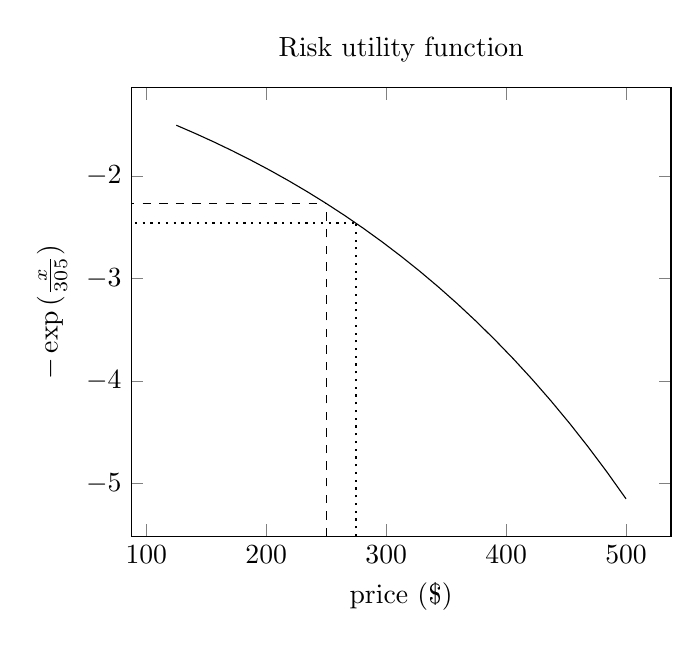
\begin{tikzpicture}[domain=125:500]
        \begin{axis}[xlabel=price (\$), ylabel=$-\exp{(\frac{x}{305})}$, title=Risk utility function]
            \addplot[mark=none] {-exp(x/(1.22*250)}; 
            %\addlegendentry{$-e^{(\frac{x}{1.22*250})}$}
            \draw[dashed] (axis cs:250,\pgfkeysvalueof{/pgfplots/ymin}) -- (axis cs:250,-2.27);
            \draw[dashed] (axis cs:0,-2.27) -- (axis cs:250,-2.27);
            \draw[dotted,thick] (axis cs:275,\pgfkeysvalueof{/pgfplots/ymin}) -- (axis cs:275,-2.46);
            \draw[dotted,thick] (axis cs:0,-2.46) -- (axis cs:275,-2.46);
        \end{axis}
    \end{tikzpicture}
    \caption{Risk-utility function of passenger}
    \label{fig:RiskUtilityFunctionOfPassenger}
\end{figure*}

After determining the risk-utility function of a passenger, the model can calculate the utility of other situations. It can do so by calculating the utility of a certain set $S = \left\{ p_1, p_2, \ldots, p_n\right\}$ where $p_n$ is a possible future price with probability $P^{p_n}$ of occurring using the following formula.
$$
u(S) = \sum (\forall x \in S: P^{p_n} \times -e^{x/R})
$$

The price a passenger is than willing to pay is the inverse of this utility:
$$
u^{-1}(u(S)) = R \log(-u(S))
$$

In the base case for the simulation the risk premium is set at a level of 10~percent. 
$$RP = 0.1$$

This thus implies that the customer is willing to pay 10~percent more for the same ticket in the hypothetical situation to prevent uncertainties, which seems like a reasonable amount in a realistic setting.


\parameter{the passenger's likelihood of travelling \hfill ($P^f = 0.5$)}
The passenger's likelihood of travelling represents the probability of the passenger actually wanting to buy a flight ticket at the time of maturity. This parameter $P^f$ is a value between 0 and 1, which represent \emph{certainly \textbf{not} flying} and \emph{certainly flying} respectively. At the time of computing the passenger's WTP, the passenger \emph{does} know the exact value of this variable.

Whether the passenger actually decides to fly at maturity is simulated by drawing a random variable from a uniform distribution $r^f = U(0,1)$. When $r^f \le P^f$ the passenger decides to fly, and when $r^f > P^f$ he decides not to do so. Whether the passenger actually wants to exercise the option thus depends on the outcome of this simulation, and whether the strike price $p_S$ is lower than the airfare at maturity (i.e., $p_S < p_{t+m}$).

During the base case of the simulation, the passenger's likelihood of flying is defined as:
$$P^f = 0.5$$

This thus means that each passenger has a 50~percent probability he has decided to actually fly at the date of maturity, and a 50~percent change he will not do so.


\parameter{the passenger's forecasting technique \hfill (historical data)}
Like the seller, the passenger also uses a certain mechanism to make predictions of the airfare at time of maturity. In the base case of the simulation, the passenger will use historical prices to make his own forecast. These data come from the training set acquired during the data collection phase (see \todo{ref}).

When the customer wants to determine the expected airfare at maturity of a certain flight, he looks up all historical price changes for flights on that same route. Next, he uses this empirical distribution to determine the probabilities of certain price movements.

As an example, consider a customer that wants to decide whether he will buy an option for the flight from AMS to JFK with a maturity of 3~days at 14~days before departure. To make his forecast, he will lookup all the historical airfares of the route AMS to JFK at 14~days prior to departure in the training set, and compare these with all the fares 3~days later. The passenger will thereby thus get an empirical distribution with relative price changes of an exact same option in the historical dataset. This series will then, in combination with the passenger's risk utility, be used to compute the customer's forecast.


\subsubsection{General characteristics of the simulation model}
Next to the parameters and assumptions specific to the four entities described previously, the simulation model itself also has some characteristics defined.

\parameter{arrival rate of passengers \hfill ($(42 - m) \times n$)}
As seen in the process description of the simulation (see \todo{ref}), the model will generate passengers to determine the performance of the model. A passenger will arrive at every day before the departure of the flight for the full observed 42~days. However, it is only possible for a passenger to buy an option with $m$ days to maturity up till $m$ days before departure. The number of customer arrivals per flight is thus fixed per simulation and can be expressed as $42 - m$.

For each specific route with $n$ flights, the simulation will therefore generate $(42 - m) \times n$ passengers.

\parameter{number of trials \hfill (N=150)}
Because pseudo random generation of numbers and probabilities are used in this model, there is a possibility of generating outliers in only a single run. To prevent such scenarios from happening, every simulation is run a vast amount of times. The acquired data from these multiple trials is then averaged to get the converged mean.

The convergence plot of three example flights is shown in \autoref{fig:ConvergencePlotMultiple}. As can be seen in the figure, the mean seems to stabilize at around 150~trials. This research will therefore use the average of 150~trials for every simulation.

\begin{figure*}
\centering
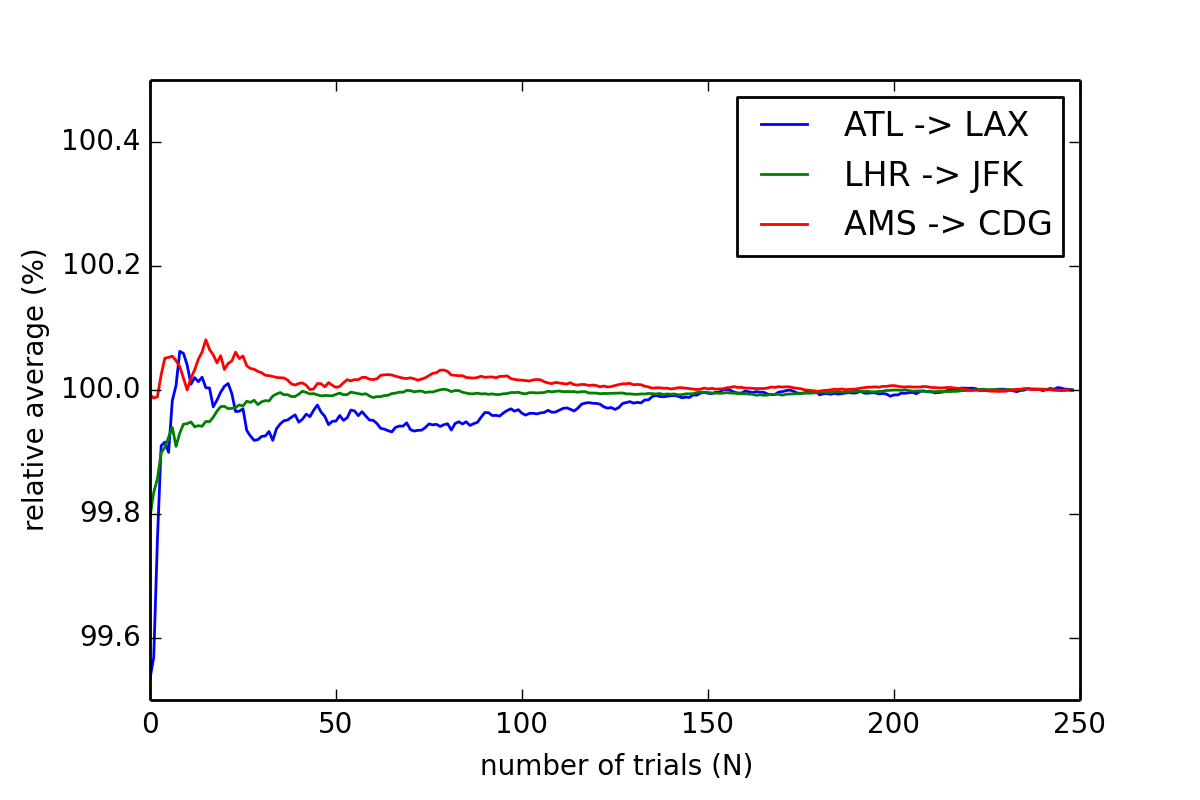
\includegraphics[width=0.8\textwidth]{figures/ConvergencePlot_multiple}
\caption{Convergence plot}
\label{fig:ConvergencePlotMultiple}
\end{figure*}
